\section{Merge Sort}
\label{sec:merge-sort-teo}

Desenvolvido por \href{https://en.wikipedia.org/wiki/John_von_Neumann}{Jon Von Neumann} em 1945, o \textit{Merge Sort} é um algoritmo de \href{https://en.wikipedia.org/wiki/Divide-and-conquer_algorithm}{dividir para conquistar}, que subdivide uma lista em singletons e os mescla em sublistas ordenadas até que exista apenas uma sublista, esta sublista é a lista original ordenada. Imagine o seguinte caso:

Você tem um baralho de cartas e gostaria de organizá-lo, seguindo o conceito do \textit{Merge Sort} você trabalha da seguinte forma:
\begin{itemize}
	\item \textbf{Divisão:} Primeiro você divide o baralho em dois baralhos menores. Cada um desses baralhos é dividido novamente até que cada sub-baralho tenha uma carta.
	\item \textbf{"Merge" (Mescla):} Nesse momento, com cada sub-baralho com uma carta, todos estão ordenados, então você começa a juntar os sub-baralhos comparando duas cartas de cada baralho e colocando-as em ordem crescente. Assim dois grupos de uma carta se tornam um baralho de duas cartas ordenadas. Em seguida, dois baralhos de duas cartas são mesclados para formar um baralho de quatro cartas, e assim por diante, até que todas as cartas estejam combinadas novamente, mas agora ordenadas.
\end{itemize}
\begin{figure}[!ht]
	\centering
	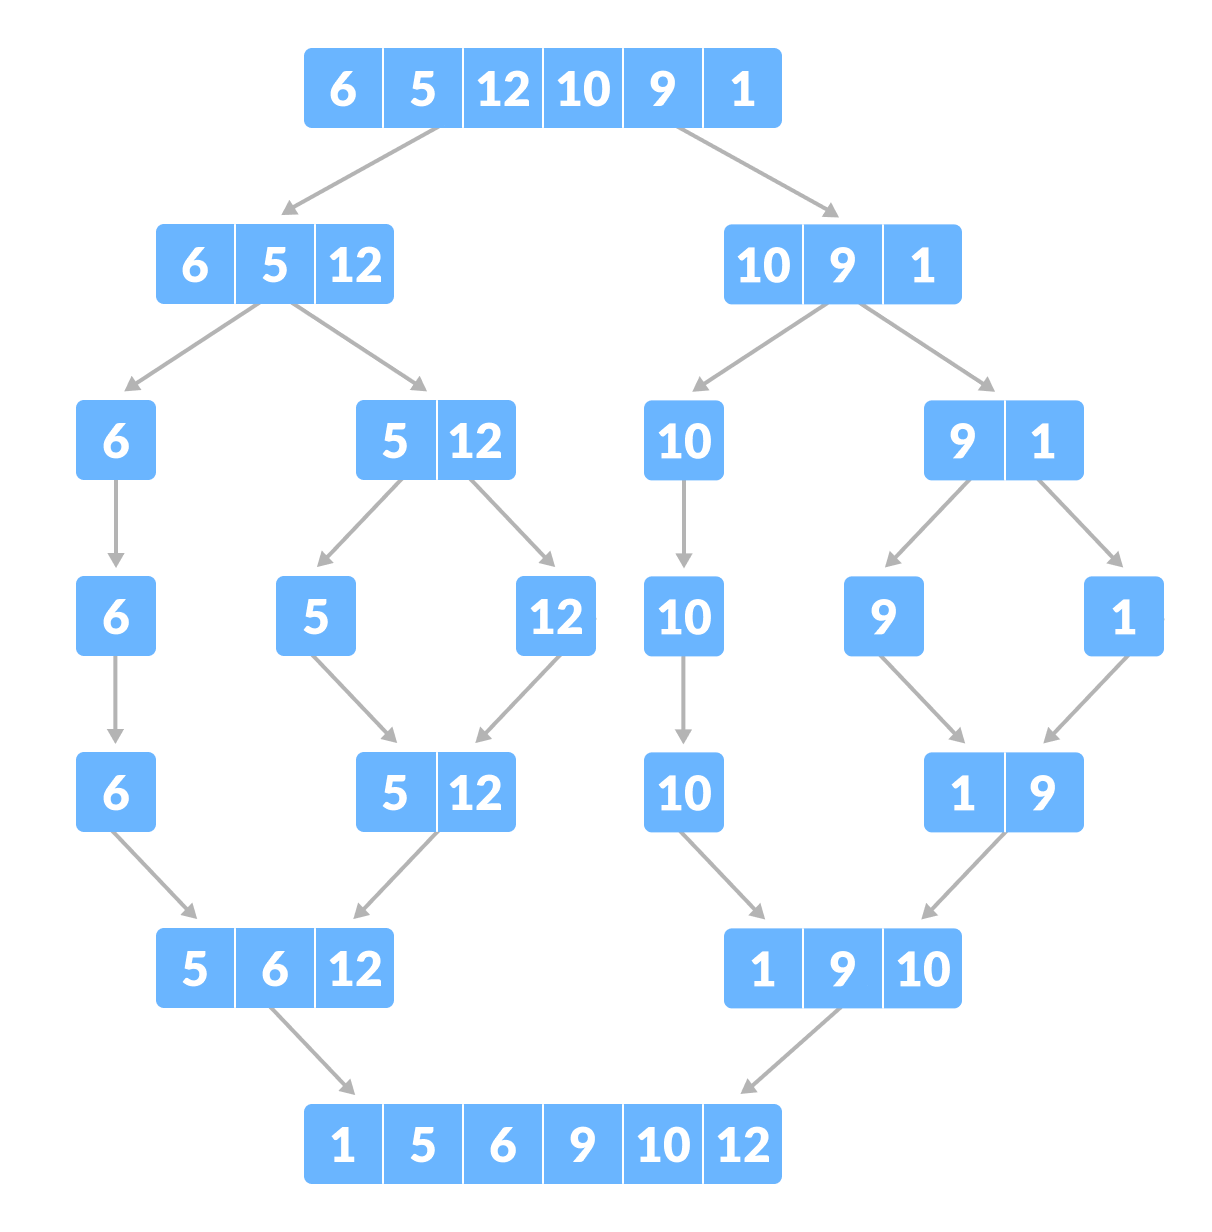
\includegraphics[scale=0.4]{figures/merge-sort-example_0.png}
	\caption{Diagrama exemplo de um Merge Sort}
	\label{fig:merge_sort_example_0}
\end{figure}

\FloatBarrier

\newpage

\subsection{Merge Sort Recursivo}

Dito isso, agora fica mais fácil estabelecer o pseudocódigo na forma recursiva. O caso base será se a lista tem no máximo elemento, pois já está ordenada. No caso recursivo, pelo teorema da recursão temos acesso ao "caso anterior", ou seja a primeira metade e segunda metade da lista original ordenadas, portanto, podemos mesclá-las.

\begin{algorithm}
	\label{algo:merge_sort_pseudo}
	\begin{algorithmic}[1]
		\Require{$\mathbf{lista}  = x_0, x_1, \ldots, x_{N-1}$}
		\Function{MergeSort}{$\mathbf{lista}$}
		\If{tamanho da \textbf{lista} $\leq 1$} \Return
		\EndIf
		\State \Return {Merge(MergeSort($1^a$ metade da \textbf{lista}), MergeSort($2^a$ metade da \textbf{lista})}
		\EndFunction
	\end{algorithmic}
\end{algorithm}

\FloatBarrier

\subsection{Merge Sort Iterativo}

\textbf{TODO}

\subsection{Função auxiliar Merge}

\noindent
Nos resta agora apenas definir a função \textbf{Merge}, que vai ser responsável por mesclar duas listas que estão ordenadas. Para tal, a função deve comparar um elemento da primeira lista com um da segunda e anexar o menor elemento entre os dois no final da lista resultado. Por exemplo:

\begin{figure}[!ht]
	\centering
	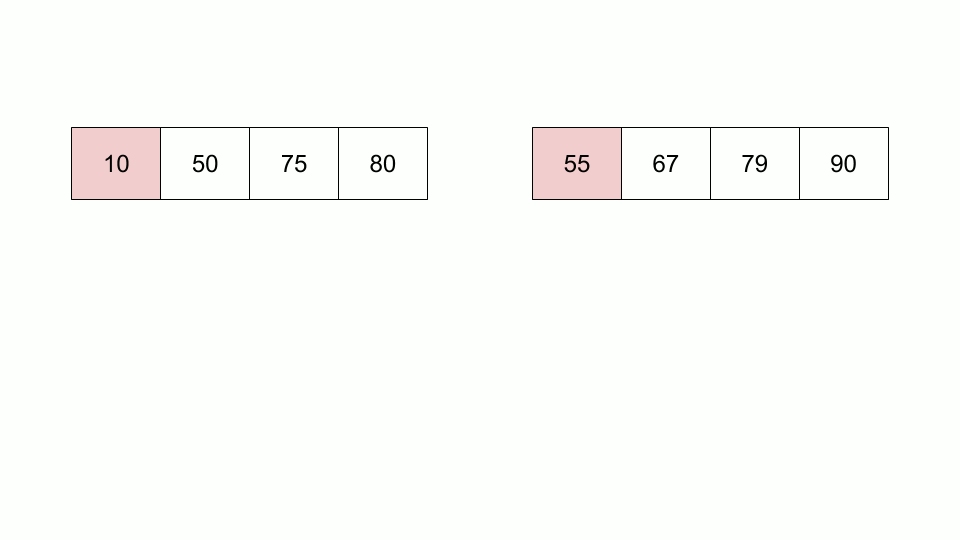
\includegraphics[scale=0.3]{figures/merge/merge-function-1.png}
	\caption{Comparando o primeiro elemento da primeira lista com o primeiro da segunda}
\end{figure}
\begin{figure}[!ht]
	\centering
	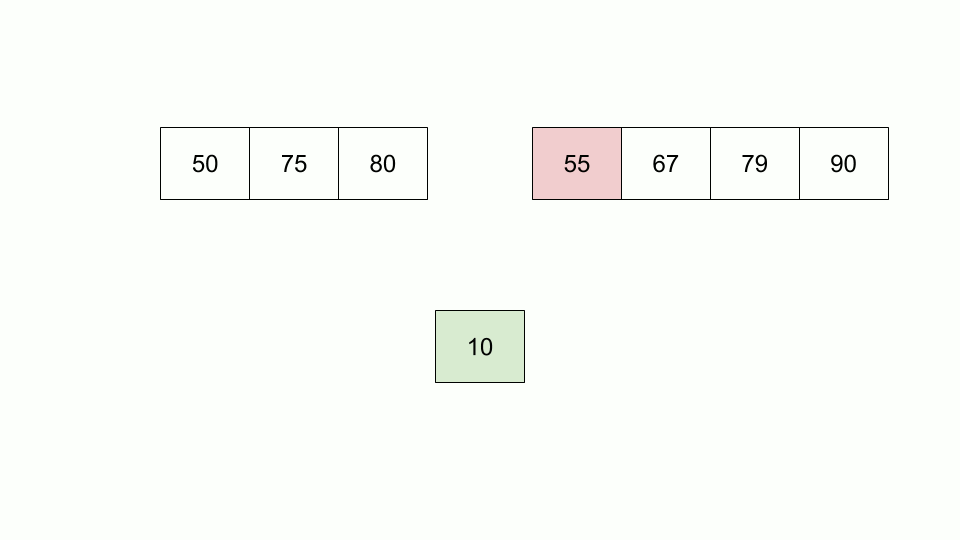
\includegraphics[scale=0.3]{figures/merge/merge-function-3.png}
	\caption{10 é menor que 55, então é anexado no final da lista resultado}
\end{figure}
\begin{figure}[!ht]
	\centering
	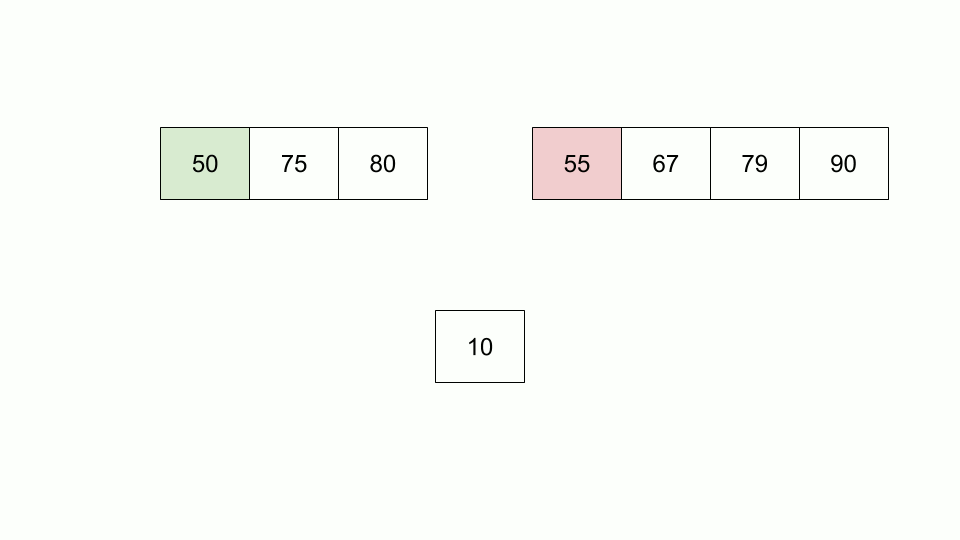
\includegraphics[scale=0.3]{figures/merge/merge-function-5.png}
	\caption{Comparando o próximo elemento da primeira lista}
\end{figure}
\begin{figure}[!ht]
	\centering
	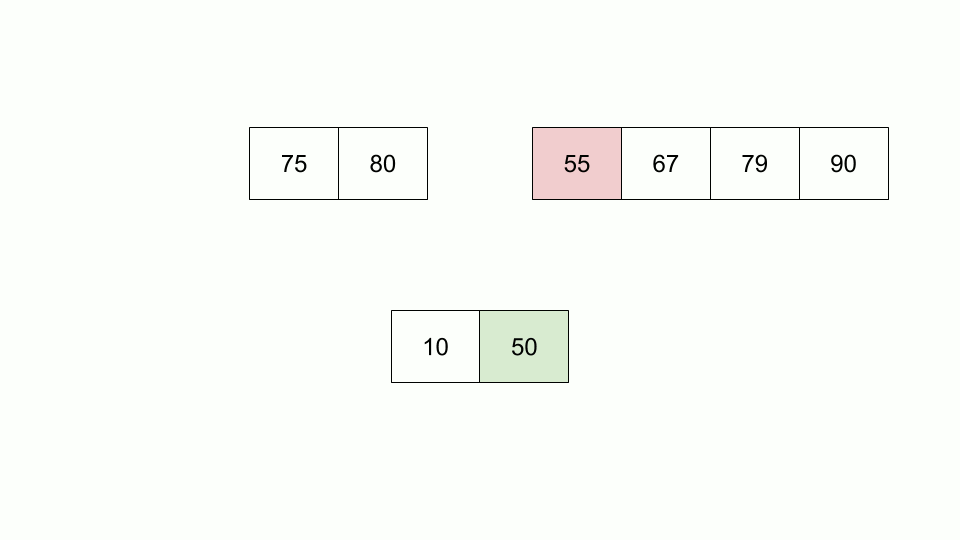
\includegraphics[scale=0.3]{figures/merge/merge-function-6.png}
	\caption{50 é menor que 55, então é anexado no final da lista resultado}
\end{figure}
\begin{figure}[!ht]
	\centering
	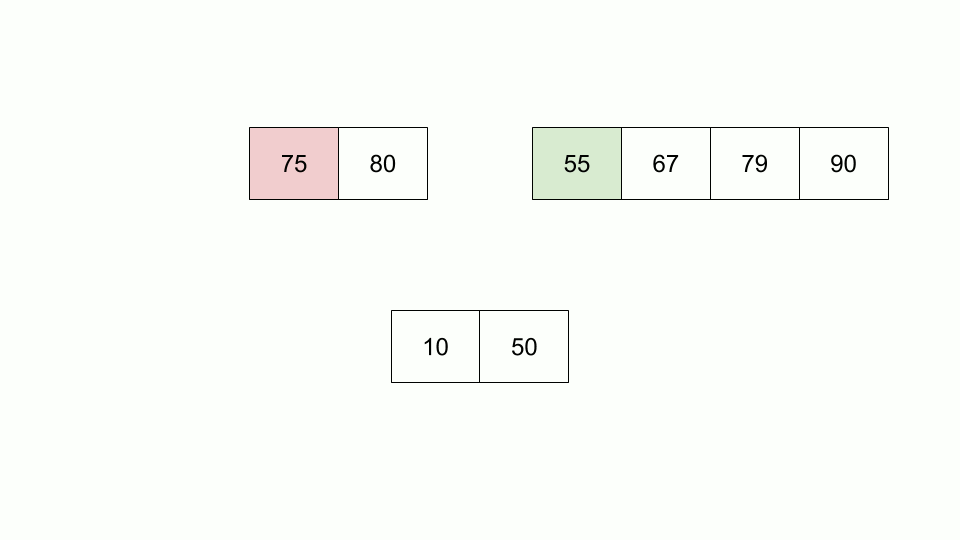
\includegraphics[scale=0.3]{figures/merge/merge-function-8.png}
	\caption{Comparando o próximo elemento da primeira lista}
\end{figure}
\begin{figure}[!ht]
	\centering
	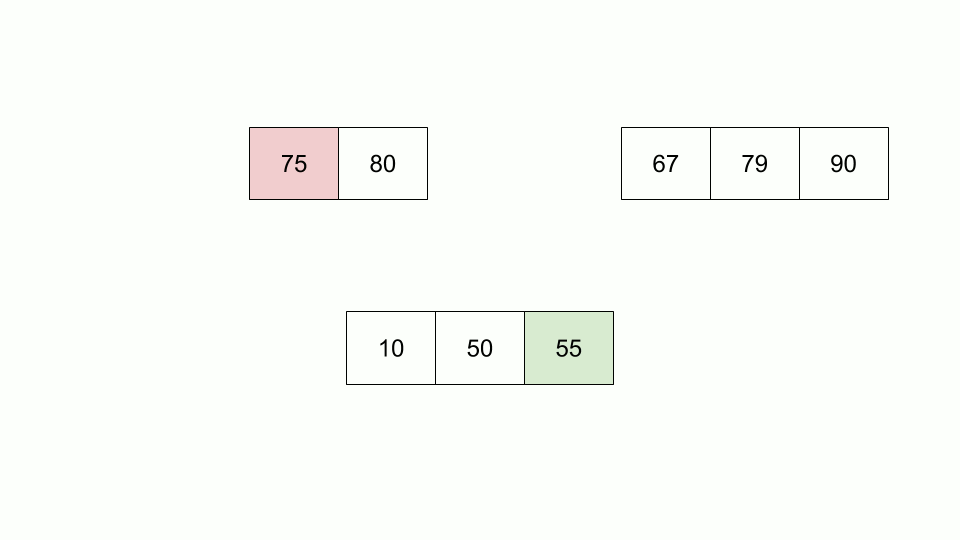
\includegraphics[scale=0.3]{figures/merge/merge-function-9.png}
	\caption{55 é menor, então é anexado no final da lista resultado}
\end{figure}
\begin{figure}[!ht]
	\centering
	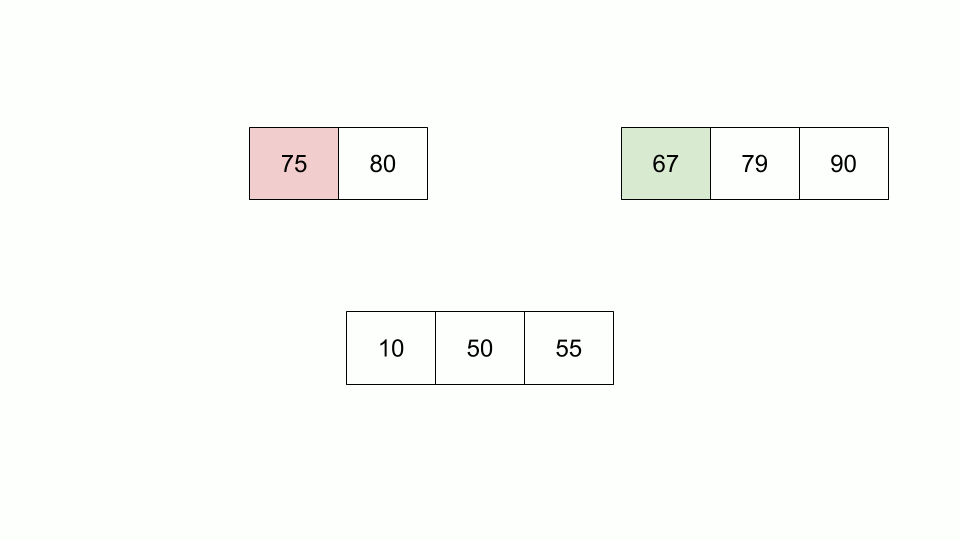
\includegraphics[scale=0.3]{figures/merge/merge-function-11.png}
	\caption{Comparando o próximo elemento da segunda lista}
\end{figure}

\FloatBarrier

E o algoritmo vai continuar até que a lista resultado esteja completa com os elementos da primeira e segunda lista.

Dito isso, construímos o pseudocódigo dessa função da seguinte forma:

\begin{algorithm}
	\label{algo:merge_aux_pseudo}
	\begin{algorithmic}[1]
		\Require{$\mathbf{listaEsquerda} = x_0, x_1, \ldots, x_{N - 1}$, $\mathbf{listaDireita} = y_0, y_1, \ldots, y_{M - 1}$}
		\Ensure{A \textbf{listaResultado} ordenada com os elementos da \textbf{listaEsquerda} e \textbf{listaDireita}}
		\Statex
		\Function{Merge}{$\mathbf{listaEsquerda}$, $\mathbf{listaDireita}$}
		\State $E, D, R = 0$ \Comment Esses serão os indexadores de cada lista
		\State $\mathbf{listaResultado} = 0, 0,\ldots, 0$
		\While{$E < N$ e $D < M$}
		\If{\textbf{listaEsquerda}(E) < \textbf{listaDireita}(D)}
		\State $\mathbf{listaResultado}(R).push(\mathbf{listaDireita}(D)$)
		\State $E = E + 1$ \Comment Partimos para o próximo elemento
		\Else
		\State $\mathbf{listaResultado}(R).push(\mathbf{listaEsquerda}(D)$)
		\State $D = D + 1$
		\EndIf
		\State $R = R + 1$
		\EndWhile
		\State $\rhd \text{ Como uma das listas vai esgotar primeiro que a outra, copiamos os elementos}$
		\State $\text{restantes para a }\mathbf{listaResultado}$
		\While {\textbf{listaEsquerda} ou \textbf{listaDireita} tiver elementos}
		\State adicione os elementos na \textbf{listaResultado}
		\EndWhile
		\State \Return \textbf{listaResultado}
		\EndFunction
	\end{algorithmic}
\end{algorithm}

\subsection{Análise de complexidade}

Dada as duas versões do \textit{Merge sort}, analisemos então suas respectivas complexidades.

\subsubsection{Análise da versão iterativa}

\textbf{TODO}

\subsubsection{Análise da versão recursiva}

\textbf{TODO}

%  TODO:
% - Análise de complexidade
